\providecommand{\main}{..}
\documentclass[\main/main.tex]{subfiles}

\begin{document}
\section{这里是第一章的标题}
\zhlipsum[8-9]
\begin{figure}[htb!]
  \centering
  \subfloat[子图1]{
\includegraphics[width = 0.45\linewidth]{figures/test_2.jpg} \label{子图1}}\hspace{0.04\linewidth}
  \subfloat[子图2]{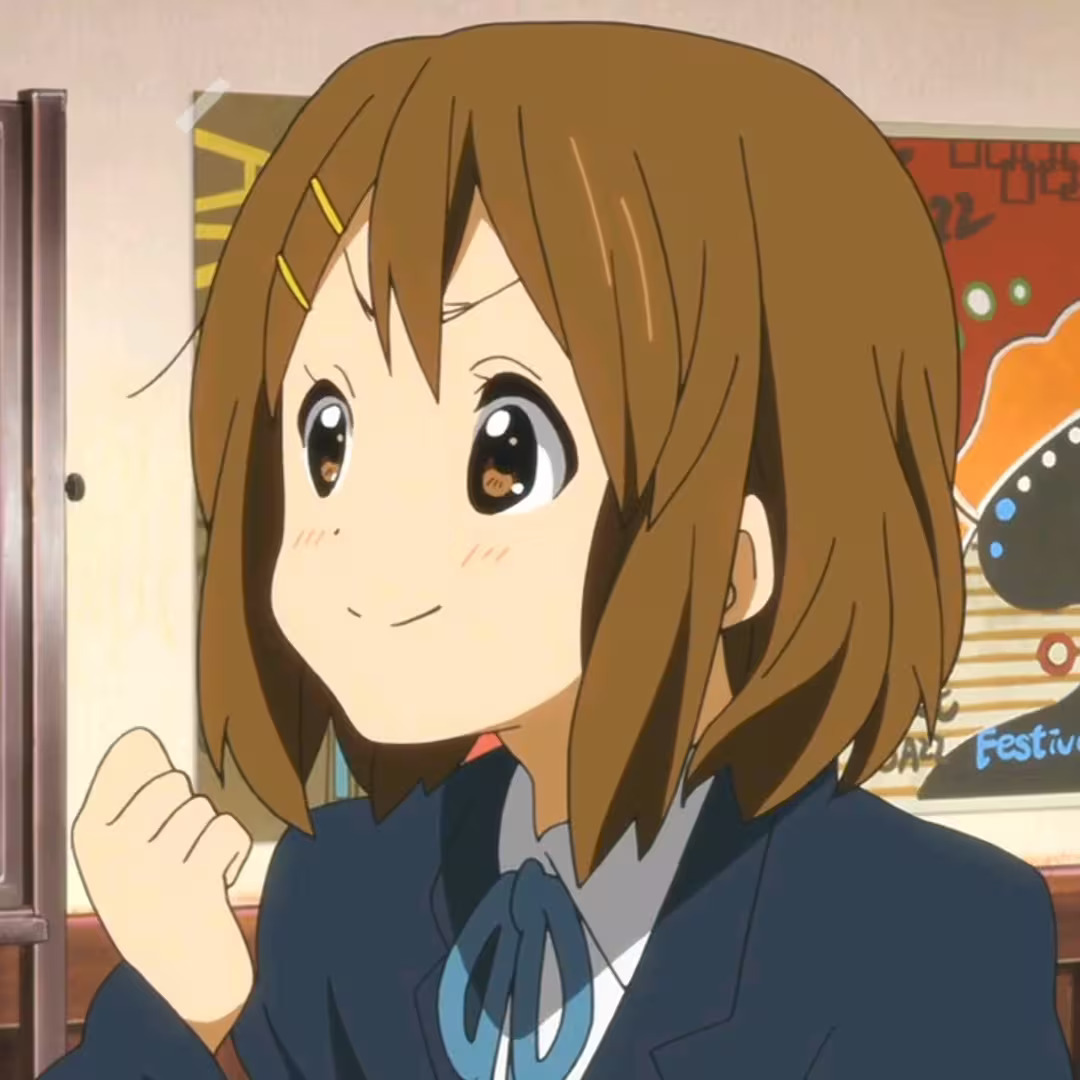
\includegraphics[width = 0.45\linewidth]{figures/test_3.jpg} \label{子图2}}
  \caption{这里是一张测试图片\cite{makise2010time}}
  \label{子图测试}
\end{figure}

\Cref{子图测试} 以及 \cref{子图1} 和 \cref{子图2} 用于测试子图的引用。\Cref{不同材料在各温度下的热导率与电阻率} 用于测试表格的引用。\Cref{eq:example} 用于测试公式的引用。

\subsection{这里是第一章的二级标题}
这里的一段话用于集中测试参考文献的引用\cite{izumi2016ero, takanashi2012eye, yano2020game},比如可以这样引用\cite{nishimiya2016voice},也可以这样引用\cite{rem2019maid, izumi2016ero, aqua2022idols}。

\subsubsection{这里是第一章的三级标题}

\begin{table}[htbp]
\centering
\caption{不同材料在各温度下的热导率与电阻率}
\label{不同材料在各温度下的热导率与电阻率}
\begin{tabular}{ll c c c}
\toprule
\multirow{2}{*}{材料} & \multirow{2}{*}{温度 (\unit{K})} & 
\multicolumn{2}{c}{热导率 $\lambda$ (\unit{W/(m\cdot K)})} &
\multirow{2}{*}{电阻率 $\rho$ (\unit{\mu\ohm\cdot \m})} \\
\cmidrule(lr){3-4}
 & & 实验值 & 理论值 &  \\
\midrule
\multirow{3}{*}{铜 (Cu)} 
 & 100 & \num{401.2} & \num{398.5} & \num{0.021} \\
 & 200 & \num{389.5} & \num{385.0} & \num{0.026} \\
 & 300 & \num{385.0} & \num{383.2} & \num{0.034} \\
\midrule
\multirow{3}{*}{铝 (Al)} 
 & 100 & \num{237.0} & \num{235.5} & \num{0.028} \\
 & 200 & \num{235.5} & \num{234.8} & \num{0.031} \\
 & 300 & \num{237.5} & \num{236.0} & \num{0.037} \\
\midrule
\multirow{3}{*}{银 (Ag)} 
 & 100 & \num{429.0} & \num{427.5} & \num{0.016} \\
 & 200 & \num{419.5} & \num{418.0} & \num{0.019} \\
 & 300 & \num{415.0} & \num{413.8} & \num{0.022} \\
\bottomrule
\end{tabular}
\end{table}

\zhlipsum[10-13]

\begin{equation}\label{eq:example}
\begin{aligned}\frac{\partial\Psi^*}{\partial t}\Psi+\Psi^*\frac{\partial\Psi}{\partial t}&=-\frac{i\hbar}{2m}\left(\frac{\partial^2}{\partial x^2}\Psi^*\right)\Psi+\frac i\hbar V\Psi^*\Psi-\Psi^*\frac i\hbar V\Psi+\Psi^*\frac{i\hbar}{2m}\left(\frac{\partial^2}{\partial x^2}\Psi\right)\\&=-\frac{i\hbar}{2m}\left(\frac{\partial^2}{\partial x^2}\Psi^*\right)\Psi+\Psi^*\frac{i\hbar}{2m}\left(\frac{\partial^2}{\partial x^2}\Psi\right)\\&=\frac{i\hbar}{2m}\frac\partial{\partial x}\left(\Psi^*\frac\partial{\partial x}\Psi-\Psi\frac\partial{\partial x}\Psi^*\right)\end{aligned},
\end{equation}

\zhlipsum*[14-15]

\begin{figure}[htb!]
  \centering
  \subfloat[并排子图 1]{
\includegraphics[width = 0.30\linewidth]{figures/band_1.png} \label{并排子图 1}}\hspace{0.03\linewidth}
  \subfloat[并排子图 2]{
\includegraphics[width = 0.30\linewidth]{figures/band_2.png} \label{并排子图 2}} \\[0.03\linewidth]
  \subfloat[并排子图 3]{
\includegraphics[width = 0.30\linewidth]{figures/band_3.png} \label{并排子图 3}}\hspace{0.03\linewidth}
  \subfloat[并排子图 4]{
\includegraphics[width = 0.30\linewidth]{figures/band_4.png} \label{并排子图 4}}
  \caption{并排子图测试}
  \label{并排子图测试}
\end{figure}

\zhlipsum*[16-17]

\end{document}